\documentclass[8pt]{beamer}

\usepackage[latin1]{inputenc}
\usepackage{graphicx}
\usepackage{colortbl}
\usepackage{tikz}
\usepackage{amsmath, amsfonts, amssymb, amsthm}
\usepackage{bm}
\usepackage{bbm} 

% \geometry{paperwidth=140mm,paperheight=105mm}
\usetikzlibrary{positioning} % Include positioning library

\usetheme{CambridgeUS}
\usecolortheme{default}
\setbeamercolor{block title}{fg=black,bg=black!5!white}   
\setbeamercolor{block title alerted}{bg=black!5!white}   

\author[Connor Braun]{Connor Braun}
\institute[]{Queen's University\\Dept. Mathematics \& Statistics}

\AtBeginSubsection[]
{
  \begin{frame}<beamer>
    \frametitle{Layout}
    \tableofcontents[currentsection,currentsubsection]
  \end{frame}
}

\newcommand{\E}{\mathbb{E}}
\newcommand{\mbb}[1]{\mathbb{#1}}
\newcommand{\1}[1]{\mathbbm{1}_{\{#1\}}}
\newcommand{\mc}[1]{\mathcal{#1}}

\DeclareMathOperator{\iid}{i.i.d.}

\graphicspath{{./figures/}}

\begin{document}

\title[MSc Project Presentation]{Synthesis of Discrete Time Decentralized Control Models of Neuronal Networks}
\subtitle{(MSc Project Presentation)}

\begin{frame}

    \titlepage

\end{frame}

\section{Introduction}

\begin{frame}{Objective} 
    \uncover<+->{The main goal for this project is to extend neuronal network models to stochastic control.\\[5pt]}
    \uncover<+->{For a network of neurons indexed $\mc{N}=\{1,2,\dots, N\}$:}
    \begin{center}
        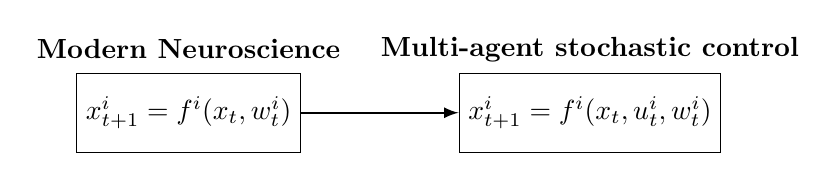
\begin{tikzpicture}

            \uncover<+->{
            \node (box1) [draw, rectangle, minimum width=2.5cm, minimum height=1cm] {$x^i_{t+1}=f^i(x_t,w^i_t)$};
            \node at (box1.north) [yshift=0.3cm] {\textbf{Modern Neuroscience}};
            }
            \uncover<+->{
            \node (box2) [draw, rectangle, minimum width=2.5cm, minimum height=1cm, right=2cm of box1] {$x^i_{t+1}=f^i(x_t,u^i_t,w^i_t)$};
            \node at (box2.north) [yshift=0.3cm] {\textbf{Multi-agent stochastic control}};
            \draw[->, thick, >=latex] (box1) -- (box2);
            }
        \end{tikzpicture}
    \end{center}
    \uncover<+->{Where $\{x_t\}_{t\geq 0}=\{(x^1_t,x^2_t,\dots,x^N_t)\}_{t\geq 0}$ is a (discrete-time) neuron state trajectory,
    and $\{w^i_t\}_{t\geq 0,i\in\mc{N}}$ is $\iid$ noise.\\[5pt]}
    \uncover<+->{{\bf The challenge}: this new model must be biologically meaningful.\\[5pt]}
    \uncover<+->{\textbf{But why stochastic control?}}
\end{frame}

\begin{frame}{Impetus}
\uncover<1->{A core goal of neuroscience is to understand {\bf neurocomputation}.\\[5pt]}
\uncover<2->{The human brain has ~100 billion neurons, operating on a continuum of spatial and temporal resultions.\\[5pt]}
\uncover<3->{\textbf{\underline{Dynamical Models}}}
\begin{columns}
    \begin{column}{0.5\textwidth}
        \begin{center}
            \only<3->{{\bf "Mechanistic"\\[5pt]}}
            \only<4-6>{\includegraphics[width=0.5\textwidth]{fig1.png}\\}
            \only<5-5>{$(N=1)$ $dX^i_t=f^i(X^i_t)dt+dB^i_t$}
            \only<6-6>{$(N>1)$ $dX^i_t=f^i(X_t)dt+dB^i_t$}
            \only<7->{\includegraphics[width=0.5\textwidth]{fig2.png}\\}
            \only<7->{$(N\rightarrow\infty)$}
        \end{center}
    \end{column}
    \begin{column}{0.5\textwidth}
        \begin{center}
            \uncover<8->{{\bf "Probabilistic"\\[5pt]}}
            \uncover<9->{\includegraphics[width=0.5\textwidth]{fig3.png}\\[12pt]}
            \uncover<10->{$P(\text{spike in $[t,t+h)$})=\lambda_tdt+o(h)$}
        \end{center}
    \end{column}
\end{columns}
\vspace{5pt}
\uncover<11->{Describe {\bf what} the network is doing quite well, but provide little insight as to \textbf{why}.\\[5pt]}
\uncover<12->{{\bf \underline{Deep learning methods}} can prescribe interpretable functions (i.e., the "{\bf why}"), but...}
\begin{itemize}
    \uncover<13->{\item lack biological realism}
    \uncover<14->{\item are analytically intractable}
    \uncover<15->{\item do not admit conditions for optimality. }
\end{itemize}
\end{frame}

\begin{frame}{Impetus ({\it continued})}
\uncover<1->{Wiener, "{\it Cybernetics: Or Control and Communication in the Animal and the Machine}" (1948).}
\begin{columns}
    \begin{column}{0.65\textwidth}
        \begin{center}
            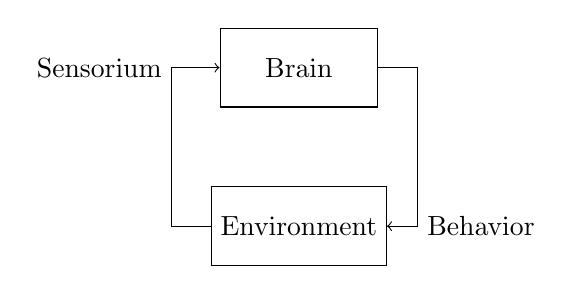
\begin{tikzpicture}
                \uncover<3->{\node (box1) [draw, rectangle, minimum width=2cm, minimum height=1cm] {Brain};
                \node (box2) [draw, rectangle, minimum width=2cm, minimum height=1cm, below=1cm of box1] {Environment};


                \draw[->] (box1.east) -- ++(0.5,0) |- (box2.east) node[midway,right] {Behavior};
                \draw[->] (box2.west) -- ++(-0.5,0) |- (box1.west) node[midway,left] {Sensorium};
                }
            \end{tikzpicture}        
        \end{center}
        \uncover<4->{\textbf{Raises several questions:}}
        \begin{itemize}
            \uncover<5->{\item can we parcelate the brain into subcontrollers?}
            \uncover<6->{\item what are the information structures?}
            \uncover<7->{\item what are the control problems?}
        \end{itemize}
        \vspace{5pt}
        \uncover<8->{{\bf Principle Hypothesis:} \underline{Brain networks} are \underline{decentralized control} systems striving to realize
        computations as optimal solutions to a set of (\underline{unknown}) control problems.\footnote{Sepulchre (2022), Burghi \& Sepulchre (2023), Ribar \& Sepulchre (2019) express a similar vision, but through the lens of classical/adaptive control in small circuits}}
    \end{column}
    \begin{column}{0.35\textwidth}
        \begin{center}
        \uncover<2->{\includegraphics[width=\textwidth]{fig4.png}}
        \end{center}
    \end{column}
\end{columns}
\end{frame}

\section{Historical Perspectives of Neuron Modeling}

\begin{frame}{Neurophysiology}
    \includegraphics[width=\textwidth]{neuron-diagram.png}
\end{frame}

\begin{frame}{Hodgkin-Huxley and Conductance-Based Models}
    \uncover<1->{\textbf{Hodgkin \& Huxley} (1952) devised what remains a gold standard biological realism.\footnote{Subsequent models such as those of Morris \& Lecar (1981), Fitzhugh (1961) and Izhikevich (2003) all share a similar philosophy, and enjoy widespread use in neuroscience.}}
    \begin{columns}
        \begin{column}{0.4\textwidth}
            % The membrane can be modeled as an RC circuit.
            \uncover<2->{\begin{center}
                \includegraphics[width=\textwidth]{fig5.png}
            \end{center}}
        \end{column}
        \begin{column}{0.6\textwidth}
           \begin{itemize}
            \uncover<3->{\item $(i)$: $I(t)$, total input current}
            \uncover<4->{\item $(ii)$: $I_C(t)=C_mdV^i_t/dt$, current across capacitor}
            \uncover<5->{\item $(iii)$: $I_\ell(t)=g^i_\ell(V^i_t-E_\ell)$, leak current}
            \uncover<6->{\item $(iv)$: $I_K(t)=g^i_K(m^i_K(t))^4(V^i_t-E_K)$, $K^+$ current}
            \uncover<7->{\item $(v)$: $I_{Na}(t)=g^i_{Na}(m_{Na}(t))^3h_{Na}(t)(V^i_t-E_{Na})$, $Na^+$ current}
           \end{itemize} 
        \end{column}
    \end{columns}
    \vspace{4pt}
    \uncover<8->{{\bf Kirchoff's current law:} $I(t)=I_C(t)+I_\ell(t)+I_K(t)+I_{Na}(t)$}
    \begin{align*}
        \uncover<9->{C_m\frac{dV^i_t}{dt}&=-g_\ell(V^i_t-E_\ell)-g_{Na}(m^i_{Na}(t))^3h^i_{Na}(t)(V^i_t-E_{Na})-g_K(m^i_K(t))^4(V^i_t-E_K)+I(t)}\\
        \uncover<10->{\tau_y(V^i_t)\frac{dy}{dt}&=-y+\phi_{y,\infty}(V^i_t)}
    \end{align*}
    \uncover<11->{for $y\in\{m_{Na},m_K,h_{Na}\}$, which is a $[0,1]$-valued \textbf{gating} variable (also contained in $X^i_t$). Further, $\phi_{y,\infty}:\mbb{R}\rightarrow (0,1)$ is an equilibrium function, and $\tau_y$ is time constant.}
\end{frame}

\begin{frame}{Hodgkin-Huxley and Conductance-Based Models ({\it continued})}
    \uncover<1->{More generally, one can consider \textbf{conductance-based networks}}
    \uncover<2->{\begin{align*}
        C^i_m\frac{dV^i_t}{dt}=-I^i_\ell(V^i_t)-\sum_{k\in\mc{C}_I}I^i_k(X^i_t)-\sum_{j\in\mc{N}}I^i_j(X^i_t,V^j_t)\label{eq17}
    \end{align*}}
    \uncover<3->{where $\{\ell\}\cup \mc{C}_I$ index \textbf{intrinsic} currents, and $\{I^i_j\}_{j\in\mc{N}}$ so-called \textbf{extrinsic} currents.}\\
    \begin{columns}
        \begin{column}{0.2\textwidth}
            \uncover<4->{\begin{center}
                \includegraphics[width=\textwidth]{fig6.png}
            \end{center}}
        \end{column}
        \begin{column}{0.8\textwidth}
            \uncover<4->{\begin{align*}
                I^i_j(X^i_t,X^j_t)=u^i_jq_js^i_j(t)(V^i_t-E_j),\quad\tau(V^j_t)\frac{ds^i_j(t)}{dt}=-s^i_j(t)+\alpha_j\tau_j(V^j_t)\phi_j(V^j_t)
            \end{align*}}
            \begin{itemize}
                \uncover<5->{\item Much like the gating variables (e.g. $m^i_{Na}$, $m^i_K$, $h^i_{Na}$ in HH), $s^i_j\in X^i_t$ are $[0,1]$-valued and have an almost identical physiological interpretation.}\\
                \uncover<6->{\item $q_j\in\{-1,1\}$ is the synaptic polarity, and $u^i_j$ are called \textbf{synaptic weights}.}
            \end{itemize}
        \end{column}
    \end{columns}
    \vspace{8pt}
    \uncover<7->{Key points:}
    \begin{itemize}
        \uncover<8->{\item Dynamics are of the general form $dX^i_t=\left(f^i(X^i_t)+\sum_{j\in\mc{N}}u^i_jg_j(X^i_t,X^j_t)\right)dt+\sigma^i(X^i_t)dB^i_t$ \footnote{Faisal et al., 2008 review the ubiquity of noise in membrane potential dynamics; here, the gates and synapses are deterministic since they are mean field representations of channel protein populations.}}
        \uncover<9->{\item Spiking is \textbf{implicit} in the trajectory of $(X^i_t)_{t\geq 0}$ -- poor mathematical structure.}
    \end{itemize}
\end{frame}

\begin{frame}{Integrate-and-Fire (IF) Methods}
    \uncover<1->{\textbf{Original model:} Lapicque (1907), Knight (1972); \textbf{"Derivation" from HH}: Kistler et al. (1997); \textbf{Predicting spike times of CB models and real neurons:} Jolivet et al. (2004, 2006).}\\[5pt] 
    \uncover<2->{Modify or remove the intrinsic dynamics facilitating spikes ($Na^+$, $K^+$-currents).}\\[5pt]
    \uncover<3->{Impose an artificial spiking criterion: for $i\in\mc{N}$, $T^i_0:=0$ and}
    \begin{align*}
        \uncover<3->{T^i_{n+1}:=\inf\{t\geq T^i_n+\delta:V^i_t\geq\vartheta^i\},\quad n\geq 0}
    \end{align*}
    \uncover<4->{where $\delta>0$ is an \textbf{absolute refractory period} and $\vartheta^i\in\mbb{R}$ is a \textbf{fixed threshold}. Then, for $A\in\mc{B}(\mbb{R}_+)$, define the point measure}
    \begin{align*}
        \uncover<5->{Z^i_t(A):=\sum_{m=1}^{M^i}\delta_{T^i_m}(A)} 
    \end{align*}
    \uncover<6->{with $M^i$ the number of spikes emitted by unit $i$ over $\mbb{R}_+$.\footnote{$M^i$ is at-most countable due to $\delta>0$, but verifying $M^i=\infty$ $a.s.$ is nontrivial, in general (Buonocore et al., 2015).}}\\[5pt] 
    \uncover<7->{Voltage dynamics are given by the stochastic differential equation:}
    \begin{align*}
        \uncover<8->{dV^i_t=\left(f^i(V^i_t)dt+\sum_{j\in\mc{N}\setminus\{i\}}u^i_j\int_0^th^i_j(t-s)Z^j(ds)\right)dt+\sigma^i(V^i_t)dB^i_t-V^i_{t-}Z^i(dt),\quad i\in\mc{N}}
    \end{align*}
    \uncover<9->{where the $h^i_j$ are {\bf synaptic kernels}, and $V^i_{t-}:=\lim_{s\nearrow t}V^i_s$. The last term is a post-spike reset.}
\end{frame}

\begin{frame}{Integrate-and-Fire (IF) Methods ({\it continued})}
    \begin{center}
    \begin{tikzpicture}
        \node [draw, rectangle, minimum width=4cm, inner sep=8pt] (box) {
        \begin{minipage}{0.95\textwidth}
            \textbf{Example} [Leaky IF (LIF) Network Model]\\[5pt]
            \uncover<2->{Only the leak current is retained; neurons are given as coupled Ornstein-Uhlenbeck processes (with resets):}\\
            \begin{align*}
                \uncover<3->{dX^i_t&=\left(-g_\ell(V^i_t-E_\ell)+\sum_{j\in\mc{N}}u^i_j s_j(t)\right)dt+\sigma^i(X^i_t)dB^i_t-V^i_{t-}Z^i(dt)}\\
                \uncover<4->{\frac{s_j(t)}{dt}&=-s_j+\sum_{n:T^j_n\leq t}\delta(t-T^j_n)}
            \end{align*}           
        \end{minipage}
        };
    \end{tikzpicture}
    \end{center}
    \begin{itemize}
        \uncover<5->{\item While spiking processes $Z^i_t:=Z^i([0,t))$ is made explicit in IF-type models, it is only related to the processes $V_t$ through a sequence of difficult {\bf first-passage-time problems}.}
    \end{itemize}
\end{frame}

\begin{frame}{Probabilistic Models}
    \begin{itemize}
        \uncover<1->{\item "Hard" thresholds are not very realistic empirically (Koch et al., 1995) and can be relaxed in the presence of noise (Plesser \& Gerstner, 2000) through a nonnegative \textbf{stochastic intensity} process $(\lambda_t)_{t\geq 0}$}
        \begin{align*}
            \uncover<2->{P(Z^i([t,t+h])=1|\mc{F}_t)=\lambda^i_th+o(h)}
        \end{align*}
        \uncover<3->{for the filtration $\mc{F}_t$ to which the $B^i_t$, $i\in\mc{N}$ are adapted.}\\
        \uncover<4->{\item We wish for $\lambda_t$ to serve as a \textbf{link} (or profile of \textbf{excitability}) between the state $X^i_t$ and spiking $Z^i_t$ processes: $\lambda^i_t=\lambda(X^i_t)$ for some $\lambda:\mbb{R}\rightarrow\mbb{R}_+$.}
    \end{itemize}
\end{frame}

\begin{frame}{Probabilistic Models ({\it continued})}
    \uncover<1->{In fact, a significant branch of neuronal modeling is dedicated to purely probabilistic models.}
    \begin{center}
    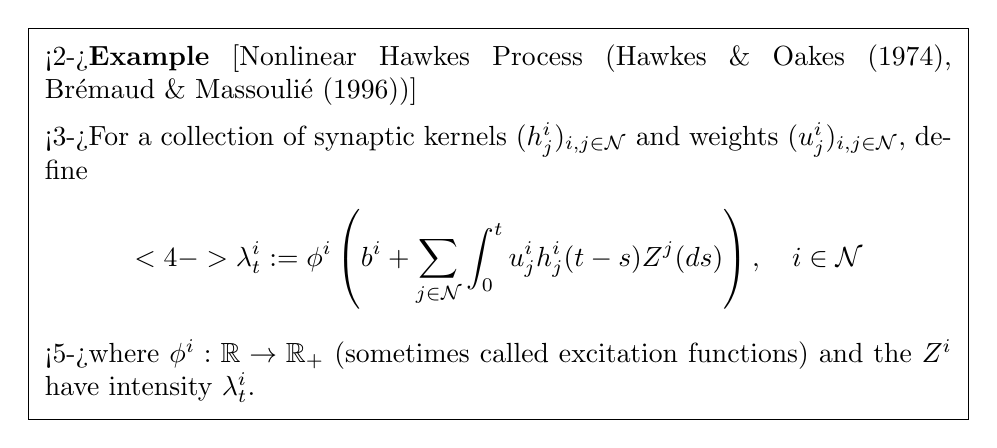
\begin{tikzpicture}
        \uncover<2->{\node [draw, rectangle, minimum width=4cm, inner sep=6pt] (box) {
        \begin{minipage}{0.95\textwidth}
            \uncover<2->{\textbf{Example} [Nonlinear Hawkes Process (Hawkes \& Oakes (1974), Br\'emaud \& Massouli\'e (1996))]}\\[5pt]
            \uncover<3->{For a collection of synaptic kernels $(h^i_j)_{i,j\in\mc{N}}$ and weights $(u^i_j)_{i,j\in\mc{N}}$, define}
            \begin{align*}
               \uncover<4->{\lambda^i_t:=\phi^i\left(b^i+\sum_{j\in\mc{N}}\int_0^tu^i_jh^i_j(t-s)Z^j(ds)\right),\quad i\in\mc{N}}
            \end{align*}
            \uncover<5->{where $\phi^i:\mbb{R}\rightarrow\mbb{R}_+$ (sometimes called excitation functions) and the $Z^i$ have intensity $\lambda^i_t$.}   
        \end{minipage}
        };}
    \end{tikzpicture}
    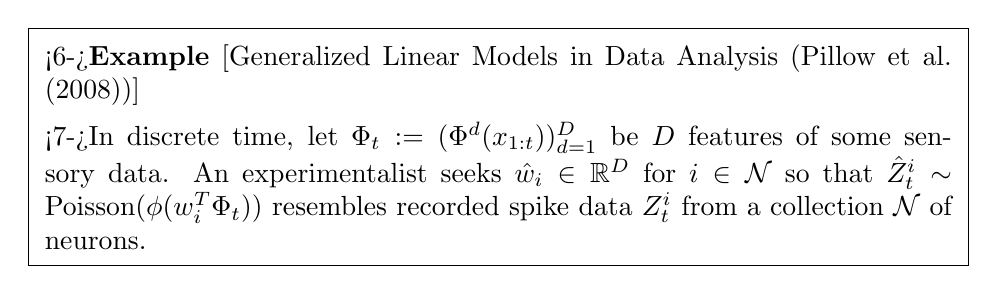
\begin{tikzpicture}
        \uncover<6->{\node [draw, rectangle, minimum width=4cm, inner sep=6pt] (box) {
        \begin{minipage}{0.95\textwidth}
            \uncover<6->{\textbf{Example} [Generalized Linear Models in Data Analysis (Pillow et al. (2008))]}\\[5pt]
            \uncover<7->{In discrete time, let $\Phi_t:=(\Phi^d(x_{1:t}))_{d=1}^D$ be $D$ features of some sensory data. An experimentalist seeks $\hat{w}_i\in\mbb{R}^D$ for $i\in\mc{N}$
            so that $\hat{Z}^i_t\sim\text{Poisson}(\phi(w_i^T\Phi_t))$ resembles recorded spike data $Z^i_t$ from a collection $\mc{N}$ of neurons.}
        \end{minipage}
        };}
    \end{tikzpicture}
    \end{center}
\uncover<8->{Summary:}
\begin{itemize}
    \uncover<9->{\item At a minimum, spiking processes must be mathematically explicit.}
    \uncover<10->{\item Probabilistic and mechanistic perspectives have complementary strengths for modelling neurodynamics.}
\end{itemize}
\uncover<11->{How can mechanistic and probabilistic models be unified sensibly?}
\end{frame}

\section{Point Processes}

\begin{frame}{Point Process Theory}{Br\'emaud (1981), Karr (1991)}
    \uncover<2->{\begin{block}{\textbf{Definition} [Point Process]}
        Let $S$ be a locally compact Polish space, and $\mc{M}(S)$ the set of Radon measures on $S$. A random measure $Z:(\Omega,\mc{F},P)\rightarrow \mc{M}(S)$ is a $S$-point process
        if $Z(A)\in\mbb{Z}_+$ for all relatively compact $A\in\mc{B}(S)$ and $Z(S)=\infty$ $P$-a.s. $Z$ is called {\bf regular} if $Z(\{x\})\leq 1$ for $x\in S$.
    \end{block}}
    \uncover<3->{On $(\mbb{R}_+,\mc{B}(\mbb{R}_+))$, $Z$ can be represented by a sequence $\{T_k\}_{k\geq 0}$ as $Z=\sum_{k\geq 1}\delta_{T_k}$, where}
    \begin{align*}
        \uncover<4->{T_0=0,\quad T_{k}=\inf(t\geq 0:Z_t:=Z([0,t])=k),\quad k\geq 1.}
    \end{align*}
    \vspace{-0.5cm}
    \uncover<5->{\begin{block}{\textbf{Definition} [Stochastic Intensity Process]}
        A nonnegative, $\mc{F}_t$-predictable process $\lambda_t$ with $\int_0^t\lambda_sds<\infty$ a.s. for any $t\geq 0$ is the stochastic intensity of a point process $Z$ on $\mbb{R}_+$ iff
        for any $\mc{F}_t$-predictable $C_t$:
        \begin{align*}
            \uncover<6->{\E\left(\int_0^\infty C_sZ(ds)\right)=\E\left(\int_0^\infty C_s\lambda_sds\right).}
        \end{align*}
    \end{block}}
    \uncover<7->{Note: integration here is in the Riemann-Stieltjes sense: $\int_0^t C_sZ(ds)=\sum_{k\geq 1}C_{T_k}\1{T_k\leq t}$.}
\end{frame}

\begin{frame}{Point Process Theory ({\it continued})}{Br\'emaud (1981), Karr (1991)}
    \uncover<+->{\begin{alertblock}{{\bf Theorem 1} [Br\'emaud (1981)]}
        If a point process $Z_t$ admits $\mc{F}_t$-intensity $\lambda_t$, then $Z_t$ is locally finite and $Z_t-\int_0^t\lambda_sds$ is a $\mc{F}_t$-local martingale.
    \end{alertblock}}
    \uncover<+->{Probabilistic neuron models correspond to this abstract notion of stochastic intensity. Let $\{S_n\}_{n\geq 1}$ be a localizing sequence, and $h>0$:}
    \begin{align*}
       \uncover<+->{\lim_{n\rightarrow\infty}\E\left(\int_{t\wedge S_n}^{t+h\wedge S_n}Z(ds)\bigg|\mc{F}_t\right)&=\lim_{n\rightarrow\infty}\E\left(\int_{t\wedge S_n}^{t+h\wedge S_n}\lambda_sds\bigg|\mc{F}_t\right)}\\
       \uncover<+->{&\Rightarrow\quad\E\left(Z_{t+h}-Z_t|\mc{F}_t\right)=\E\left(\int_t^{t+h}\lambda_sds\bigg|\mc{F}_t\right)}
    \end{align*}
    \uncover<+->{whereby the dominated convergence and Lebesgue differentiation theorems:} 
    \begin{align*}
        \uncover<+->{\lim_{h\rightarrow 0^+}\frac{1}{h}\E\left(Z_{t+h}-Z_t|\mc{F}_t\right)=\E\left(\lim_{h\rightarrow 0^+}\frac{1}{h}\int_t^{t+h}\lambda_sds\bigg|\mc{F}_t\right)=\lambda_t.}
    \end{align*}
    \uncover<+->{$\lambda_t$ can be viewed as a dynamical law governing a stochastic spiking mechanism, and we wish to prescribe particular $\lambda_t$ to individual neurons.}\\[5pt]
    \uncover<+->{This is accomplished via {\bf thinning}:}
    \begin{align*}
        \uncover<+->{Z(A):=\int_{A}\int_{\mbb{R}_+}\1{y\in[0,\lambda_s]}\Pi(dy\times ds),\quad \Pi\;\text{is standard Poisson on $\mbb{R}_+\times\mbb{R}_+$.}}
    \end{align*}
\end{frame}

\begin{frame}{Marked Point Processes}
    \uncover<+->{\begin{block}{\textbf{Definition} [Marked Point Process (MPP)]}
        Suppose that to a point process $(T_n)_{n\geq 0}$ is associated a
        sequence of $(Y,\mc{Y})$-valued random variables $(Y_n)_{n\geq 0}$. Then
        $\{(T_n,Y_n)\}_{n\geq 0}$ is called a MPP with
        marks $(Y_n)_{n\geq 0}$ and {\it mark space} $Y$.
    \end{block}}
    \uncover<+->{Predictable $\sigma$-algebra: $\mc{P}(\{\mc{F}_t\}_{t\geq 0}):=\sigma((t,\infty)\times A:t\in\mbb{R}_+,\,A\in\mc{F}_t)$.}\\[5pt]
    \uncover<+->{Marked predictable $\sigma$-algebra: $\tilde{\mc{P}}(\{\mc{F}_t\}_{t\geq 0}):=\mc{P}(\mc{F}_t)\otimes\mc{Y}$.}\\[5pt]
    \uncover<+->{\textbf{Integration} For any $(t,\omega,y)\mapsto C(t,\omega,y)$ is $\tilde{\mc{P}}(\mc{F}_t)$-measurable and $Z$ a $Y$-MPP, $E\in \mc{Y}$}
    \begin{align*}
        \uncover<+->{\int_0^t\int_EC(s,\omega,y)Z(ds\times dy):=\sum_{n\geq 1}C(T_n,\omega,Y_n)\1{T_n\leq t}\1{Y_n\in E}}
    \end{align*}
    \vspace{-0.5cm}
    \uncover<+->{\begin{block}{\textbf{Definition} [Intensity Kernels]}
        With $Z$ a $Y$-MPP adapted to $\mc{F}_t$, if $\forall A\in\mc{Y}$ the point process $Z_t(\omega,A)$ admits $\mc{F}_t$-predictable intensity $\lambda_t(\omega,A)$,
        then $Z$ admits the intensity kernel $\lambda_t(\omega, dy)$.
    \end{block}}
    \uncover<+->{\begin{alertblock}{\textbf{Theorem 2} [Br\'emaud (1981)]}
        If $C:\mbb{R}_+\times\Omega\times Y\rightarrow\mbb{R}_+$ is $\tilde{\mc{P}}(\mc{F}_t)$-measurable and $Z$ has intensity kernel $\lambda_t(dy)$, then
        \begin{align*}
            \E\left(\int_0^\infty\int_Y C(s,y)Z(ds\times dy)\right)=\E\left(\int_0^\infty\int_Y C(s,y)\lambda_s(dy)ds\right).
        \end{align*}
    \end{alertblock}}
\end{frame}

\begin{frame}{Martingale Characterization of Intensities}
    \uncover<+->{\begin{alertblock}{\textbf{Theorem 3} [Jacod (1975), Br\'emaud (1981)]}
        \uncover<+->{If for $t\geq 0$, $\int_0^t\int_Y|C(s,y)|\lambda_s(dy)ds<\infty$ $P$-a.s., then}
        \begin{align*}
            \uncover<+->{X_t:=\int_0^t\int_YC(s,y)[Z(ds\times dy)-\lambda_s(dy)ds],\quad t\geq 0}
        \end{align*}
        \uncover<+->{is a local martingale. If $\E(\int_0^t\int_Y|C(s,y)|\lambda_s(dy)ds)<\infty$, then $X_t$ is a martingale.}
    \end{alertblock}}
    \uncover<+->{The converse is true as well, leading to a martingale characterization of intensity processes:}
    \uncover<+->{\begin{alertblock}{\textbf{Theorem 4} [{Br\'emaud (1981)}]}
        Let $Z$ be a point process, $\lambda_t$ a nonnegative process, both adapted to $\mc{F}_t$. If $Z_t-\int_0^t\lambda_sds$ is a local martingale,
        then $\lambda_t$ is the intensity of $Z$. 
    \end{alertblock}}
\end{frame}

\begin{frame}
    \textbf{Proof}. Apply the monotone class theorem. For a sequence of localizing times $\{S_n\}_{n\geq 1}$,
    \begin{align*}
        \uncover<+->{&\E\left(Z_{t\wedge S_n}-\int_0^{t\wedge S_n}\lambda_udu\bigg|\mc{F}_s\right)=Z_{s\wedge S_n}-\int_0^{s\wedge S_n}\lambda_udu}\\
        \uncover<+->{\Rightarrow\qquad&\E\left(\int_{s\wedge S_n}^{t\wedge S_n}Z(du)\bigg|\mc{F}_s\right)=\E\left(\int_{s\wedge S_n}^{t\wedge S_n}\lambda_u du\bigg|\mc{F}_s\right)}\\
        \uncover<+->{\Rightarrow\qquad&\E\left(\int_0^{t\wedge S_n}\1{A}\1{u\in(s,\infty)}Z(du)\right)=\E\left(\int_0^{t\wedge S_n}\1{A}\1{u\in(s,\infty)}\lambda_udu\right)}
    \end{align*}
    \uncover<+->{which holds for any $A\in\mc{F}_s$. So the class of nonnegative processes for which
    \[\E\left(\int_0^{t\wedge S_n}C_s Z(ds)\right)=\E\left(\int_0^{t\wedge S_n}C_s\lambda_sds\right)\]
    holds includes indicators over
    \[\mc{K}=\{(s,\infty)\times A:0\leq s\leq t,\,A\in\mc{F}_s\}\]}
    \uncover<+->{generating $\mc{P}(\mc{F}_t)$. This class is closed under addition/scalar multiplication and pointwise bounded limits, whereby successively applying the monotone convergence theorem:}
    \begin{align*}
        \uncover<+->{\E\left(\int_0^{t\wedge S_n}C_s Z(ds)\right)=\E\left(\int_0^{t\wedge S_n}C_s\lambda_sds\right)\quad\Rightarrow\quad\E\left(\int_0^\infty C_sZ(ds)\right)=\E\left(\int_0^\infty C_s\lambda_sds\right).\tag*{$\qed$}}
    \end{align*}
    \uncover<+->{\textbf{Note}: An extremely similar procedure can be used to prove Theorem 2.}
\end{frame}

\begin{frame}{Spatial Thinning Theorem}
    \uncover<+->{\begin{alertblock}{\textbf{Theorem 5} Spatial Thinning [Chevallier et al., 2015, theorem B.11]}
        \uncover<+->{Let $\Pi$ be a $\mc{F}_t$-adapted standard Poisson process on $\mbb{R}_+^2$. If $\lambda_t$ is nonnegative, $\mc{F}_t$-predictable with $\int_0^t\lambda_s(\omega)ds<K_t(\omega)$,
        with $\E(K_t)<\infty$ for all $t\geq 0$, then}
        \begin{align*}
            \uncover<+->{Z(A)=\int_A\int_{\mbb{R}_+}\1{y\in[0,\lambda_t]}\Pi(dy\times dy),\quad A\in\mc{B}(\mbb{R}_+)}
        \end{align*}
        \uncover<+->{has stochastic intensity process $\lambda_t$.}
    \end{alertblock}}
    \uncover<+->{{\bf Proof} (sketch).} \uncover<+->{$\Pi$ is not a MPP -- form a sequence of restrictions $\Pi^k$ of $\Pi$ to $\mbb{R}_+\times[0,k]$, which have intensity kernel $dy$ on $[0,k]$. Define the sequence of processes}
    \[\uncover<+->{Z^k(A):=\int_A\int_{\mbb{R}_+}\1{y\in[0,\lambda_t]}\Pi^k(dy\times dt),\quad A\in\mc{B}(\mbb{R}_+).}\]
    \uncover<+->{It can be shown that $\1{y\in[0,\lambda_t(\omega)]}(t,\omega,y)$ is $\tilde{\mc{P}}_k(\mc{F}_t)$-measurable for any $k$, and $\int_0^t\int_{[0,k]}\1{y\in[0,\lambda_s]}dyds<K_t<\infty$ a.s. Thus, for $k\geq 1$ the process}
    \begin{align*}
        \uncover<+->{X^k_t:=\int_0^t\int_{Y_k}\1{y\in[0,\lambda_s]}\left[\Pi^k(dy\times ds)-dyds\right]&=Z^k_t-\int_0^t\min(\lambda_s,k)ds}
    \end{align*}
    \uncover<+->{is a local martingale. Taking the limit as $k\rightarrow\infty$ along a localizing sequence shows $Z_t-\int_0^t\lambda_sds$ is a local martingale, so $\lambda_t$ is the intensity of $Z$ by the martingale characterization of intensities.\hfill{$\qed$}}
\end{frame}

\begin{frame}{Soft Integrate-and-Fire Network}
    \uncover<+->{\begin{alertblock}{\textbf{Theorem 6} MPP-Based Thinning [Glasserman \& Merener (2003)]}
        \uncover<+->{Let $\Pi$ be a MPP with mark space $(0,1)$ and intensity kernel $\lambda_t(dt)=\lambda dy$, where $\lambda>0$. For a $\mc{F}_t$-adapted process $X_t$, if $0\leq\phi(x)<\lambda$ for all $x\in\mbb{X}$ then}
        \begin{align*}
            \uncover<+->{Z_t:=\int_0^t\int_{(0,1)}\1{y<\frac{1}{\lambda}\phi(x_{s-})}\Pi(dy\times ds)}
        \end{align*}
        \uncover<+->{is a $\mc{F}_t$-adapted point process with intensity $\phi(x_{t-})$.}
    \end{alertblock}}
    \uncover<+->{Rather than impose a hard threshold and refractory period on each unit (where the voltage and spiking are difficult to interrelate) define the {\bf spiking processes}}
    \begin{align*}
        \uncover<+->{Z^i(A):=\int_A\int_{\mbb{R}_+}\1{y\leq \lambda^i_t}\Pi^i(dy\times ds),\quad A\in\mc{B}(\mbb{R}_+),\;i\in\mc{N}}
    \end{align*}
    \uncover<+->{with $\{\Pi^i\}_{i\in\mc{N}}$ a set of i.i.d. standard Poisson processes on $\mbb{R}_+^2$.}\\[5pt]
    \uncover<+->{Setting $dR^i_t=dt-R^i_{t-}Z^i(dt)$, we can set $\lambda^i_t=\lambda^i(V^i_t)\1{R^i_t\geq\delta}$ (for example)
    to instantiate refractory periods.\footnote{Refractory periods of this kind were studied separately by Chevallier et al. (2015) (mean field dynamics) and Borovkov et al. (2014) (stability results) in the probabilistic setting.}}\\[5pt]
    \uncover<+->{\textbf{Soft IF Network Model}}
    \begin{align*}
        \uncover<+->{V^i_t=V^i_0+\int_0^tf^i(X^i_s)ds+\int_{0}^{t}\sigma^i(X^i_t)dB^i_s+\sum_{j\in\mc{N}}u^i_j\int_0^th^i_j(t-s)Z^j(ds)-\int_0^tV^i_{s-}Z^i(ds)}
    \end{align*}
\end{frame}

\begin{frame}{Soft Integrate-and-Fire Network ({\it continued})}
    \uncover<+->{\underline{\textbf{Soft IF Network Model}} (SIF)}
    \begin{align*}
        V^i_t=V^i_0+\int_0^tf^i(X^i_s)ds+\int_{0}^{t}\sigma^i(X^i_t)dB^i_s+\sum_{j\in\mc{N}}u^i_j\int_0^th^i_j(t-s)Z^j(ds)-\int_0^tV^i_{s-}Z^i(ds),\quad i\in\mc{N}
    \end{align*}
    \uncover<+->{or, alternatively}
    \begin{align*}
        \uncover<+->{dX^i_t&=f^i(X^i_t)+\sigma^i(X^i_t)dB^i_t+C^i(X^i_{t-},u^i)Z(dt)}\\
        \uncover<+->{&=f^i(X^i_t)+\sigma^i(X^i_t)dB^i_t+\int_{\mbb{R}_+}\tilde{\Theta}^i(X_{t-},u^i,y)\tilde{\Pi}(dy\times dt)}\\
        \uncover<+->{&=f^i(X^i_t)+\sigma^i(X^i_t)dB^i_t+\int_{(0,1)\times\mc{N}}\Theta^i(X_{t-},u^i,y)\Pi(dy\times dt)}
    \end{align*}
    \uncover<+->{where, for example, $\Theta^i(x,u^i,y)=\sum_{j\in\mc{N}}u^i_jC^i_j(x^i)\1{y\leq \phi^j(x^j)}\1{k=j}$.}\\[5pt]
    \uncover<+->{This new class of models is a superset of nonlinear Hawkes (self-exciting) point processes, and a stochastic realization of IF methods in the following sense.}
    \uncover<+->{\begin{alertblock}{\textbf{Theorem 7} Stochastic Realization of Thresholds}
        Any nonlinear Hawkes network can be realized as a SIF network. Further, fixing thresholds $(\vartheta^i)_{i\in\mc{N}}$, and approximation bounds $\varepsilon>0$, and $\delta>\tilde{\delta}>0$, 
        there exist intensity processes $\lambda^i_t$, $i\in\mc{N}$ so that $P(Z^i(T,T+\tilde{\delta}]=1)>1-\varepsilon$ whenever $T$ is a $\vartheta^i$-crossing.
    \end{alertblock}}
\end{frame}

\begin{frame}
    \uncover<+->{\textbf{Proof}.} \uncover<+->{Claim I is clear. For the second, fix $i\in\mc{N}$ and set the intensity to satisfy the absolute refractory condition $\lambda^i_t=\phi^i(R^i_{t-},V^i_{t-})=0$ for $0\leq R^i_{t-}<\delta$.
    Then $Z^i((T,T+\tilde{\delta}])\leq 1$ almost surely.} \uncover<+->{To see this, define $\xi=\inf\{s\in(T,T+\tilde{\delta}]:Z^i_s-Z^i_T=1\}$. Then,}
    \begin{align*}
        \uncover<+->{Z^i((T,T+\tilde{\delta}])=Z^i_\xi-Z^i_T+Z^i((\xi,T+\tilde{\delta}])=1+\int_\xi^{T+\tilde{\delta}}\int_{\mbb{R}_+}\1{y\leq\phi^i(s-\xi,V^i_{t-})}\Pi^i(dy\times ds)=1.}
    \end{align*}
    \uncover<+->{With $\mc{A}:=\{(s,y)\in\mbb{R}_+^2:s\in(T,T+\tilde{\delta}],\,y\leq\phi^i(R^i_{s-},V^i_{s-})\}$, and $\mu$ the Lebesgue measure on $\mc{B}(\mbb{R}_+^2)$:}
    \begin{align*}
        \uncover<+->{P(Z^i((T,T+\tilde{\delta}])=1)=P(Z^i((T,T+\tilde{\delta}])\geq 1)=P(\Pi^i(\mc{A})\geq 1)=1-e^{-\mu(\mc{A})}.}
    \end{align*}
    \uncover<+->{Finally, take $M$ large so that $e^{-M\tilde{\delta}}<\varepsilon$, and set $\phi^i(R^i_{t-},V^i_{t-})=C$ whenever both $R^i_{t-}\geq\delta$ and $t\in(T,T+\tilde{\delta}]$ to yield the result.\hfill{$\qed$}}
\end{frame}

\begin{frame}{Soft Integrate-and-Fire Network ({\it continued})}
    \uncover<+->{The complete network dynamics are (adopting the MPP-based thinning)}
    \begin{align*}
        \uncover<+->{dX_t=f(X_t)dt+\sigma(X_t)dB_t+\int_{(0,1)\times\mc{N}}\Theta(X_{t-},u,y)\Pi(dy\times ds).}
    \end{align*}
    \uncover<+->{which is a pretty typical jump-diffusion process, except $\Theta$ is discontinuous in the marks/state.}\\[5pt]
    \uncover<+->{Models of this kind have appeared sporadically in the mathematical neuroscience literature:}
    \begin{itemize}[<+->]
        \item First instance: Giraudo \& Sacerdote (1997)
        \item An identical model appears in Jahn et al. (2011), along with empirical estimation methods
        \item A non-diffusive version was introduced by Galves \& L\"ocherbach (2013), and the authors have noted the equivalence with probabilistic methods (Schmutz et al., 2023; L\"ocherbach et al., 2019).
        \item More recently, Jabin \& Zhou (2023) have derived mean-field dynamics for networks of this kind with {\bf sparse, heterogeneous coupling}.
    \end{itemize}
  
\end{frame}

\begin{frame}{Strong Solutions of the Jump-Diffusion}
    \uncover<+->{\begin{alertblock}{\textbf{Theorem 8} Existence/Uniqueness of a Strong Solution [Ikeda \& Watanabe (1989) theorem 9.1]}
        \uncover<+->{Consider the jump-diffusion dynamics
        \begin{align*}
            dX_t=b(X_t)dt+\sigma(X_t)dB_t+\int_Yq(X_{t-},y)\Pi(dy\times dt)\tag{$\ast$}}
        \end{align*}
        \uncover<+->{where $\Pi$ is a $Y$-MPP with time-homogeneous kernel $\lambda(dy)$, finite on $Y$.} \uncover<+->{If for some $M_1,M_2>0$, $x,x_1,x_2\in\mbb{R}^d$ the coefficients satisfy
        \begin{align*}
            &\|b(x)\|^2+\|\sigma(x)\|^2+\int_\Gamma\|q(x,\gamma)\|^2\lambda(d\gamma)\leq M_1(1+\|x\|^2)\\
            &\|b(x_1)-b(x_2)\|^2+\|\sigma(x_1)-\sigma(x_2)\|^2+\int_Y\|q(x_1,y)-q(x_2,y)\|^2\lambda(dy)\leq M_2\|x-y\|^2}
        \end{align*}
        \uncover<+->{then ($\ast$) admits a unique, strong solution.}
    \end{alertblock}}
    \uncover<+->{{\bf Note:} This is to say nothing of a controlled version.}\\[5pt]
    \begin{itemize}[<+->]
        \item Rather than formulate the control problem in continuous time and then acquire a discrete-time approximation (Kushner, 2000), we acquire discrete time {\bf dynamics}
        and formulate the problem free of (potentially distracting) technicalities.
    \end{itemize}
\end{frame}

\section{Discrete Time Approximation}

\begin{frame}{Discrete Time Approximation for Jump-Diffusions}
    \vspace{-0.3cm}
    \uncover<1->{\begin{block}{\textbf{Definition} [Uniform Order $\kappa$ Strong Convergence]}
        A discrete-time approximation with (constant interpolation) $x^{h}_t$ converges strongly and uniformly with order $\kappa$ to
        the jump-diffusion solution $X_t$ on the finite horizon $[0,T]$ if $\exists C,h^\ast>0$ with
        \begin{align*}
            \E\left(\sup_{0\leq s\leq T}\|X_s-x^{h}_s\|^2\right)\leq Ch^{2\kappa}
        \end{align*} 
        whenever the time discretization $h\in(0,h^\ast)$, and where $C$ is independent of $h$.
    \end{block}}
    \uncover<2->{Let $0=t_0<t_1<\cdots t_{M_T}=T$ be an equidistant grid on $[0,T]$ and define the process}
    \begin{align*}
        \uncover<2->{x^{i,h}_{m+1}=x^{i,h}_m+f^i(x^{i,h})h+\sigma^i\sqrt{h}w^i_m+\int_{\Delta_t}\int_{(0,1)\times\mc{N}}\Theta^i(x^h_m,u^i,y)\Pi(dy\times ds),\quad i\in\mc{N}}
    \end{align*}
    \uncover<3->{where we have taken $\sigma^i(x)=\sigma^i>0$ for all $x$ and $w^i_m$ are i.i.d. standard Gaussian.}
    \vspace{-0.1cm}
    \uncover<4->{\begin{alertblock}{\textbf{Theorem 9} [Bruti-Liberati \& Platen (2005)]}
        \uncover<5->{Suppose $\{x^h_{m}\}_{m=0}^{M_T}$ is as above for some $h\in(0,1)$ and the jump-diffusion satisfies the Lipschitz and growth constraints of theorem 3.} \uncover<6->{If
        \begin{align*}
            \E(\|x^h_0\|^2)<\infty,\quad\text{and}\quad\E(\|X_0-x^h_0\|^2)\leq Ch
        \end{align*}}
        \uncover<7->{for some $C>0$, then $\{x^h_m\}_{m=1}^{M_T}$ converges strongly and uniformly with order $\kappa=1/2$ to the strong solution $X^i_t$ on $[0,T]$.}
    \end{alertblock}}
\end{frame}

\begin{frame}{Discrete Time Spiking Process}
    \uncover<+->{Denoting the marks of $\Pi$ by $\{(y_n,k_n)\}{n\geq 1}\subset(0,1)\times\mc{N}$ and $\Pi_t:=\Pi((0,1)\times\mc{N}\times[0,t])$, the synaptic interactions may be expressed}
    \uncover<+->{\begin{align}
        \int_{t_m}^{t_{m+1}}\int_{(0,1)\times\mc{N}}\Theta^i(x^h_m,u^i,y)&\Pi(dy\times ds)\notag\\
        \uncover<+->{&=\1{\Pi_{t_{m+1}}-\Pi_{t_m}\geq 1}\left(\sum_{\ell=\Pi_{t_m}+1}^{\Pi_{t_{m+1}}}\sum_{j\in\mc{N}}u^i_jC^i_j(x^{i,h}_{t_m})\1{y_\ell\leq \phi^j(x^{j,h}_{t_m})}\1{j=k_\ell}\right)\notag{}}\\
        \uncover<+->{&=:\sum_{j\in\mc{N}}u^i_jC^i_j(x^{i,h}_{t_m})Z^{j,h}_{t_m}\notag{}}
    \end{align}}
    \uncover<+->{with the \textbf{discrete time spiking} $Z^{j,h}_{t_m}=\int_{\Delta_t}\int_{(0,1)}\1{y\leq\frac{N}{\lambda}\phi^j(x^{j,h}_{t_m})}\Pi^j(dy\times dt)$, where}
    \uncover<+->{\begin{align*}
        \E\left(\int_{t_m}^{t_{m+1}}\int_{(0,1)}\1{y\leq\frac{N}{\lambda}\phi^j(x^{j,h}_{t_m})}\Pi^j(dy\times dt)\right)
        \uncover<+->{&=\E\left(\int_{t_m}^{t_{m+1}}\int_{(0,1)}\1{y\leq\frac{N}{\lambda}\phi^j(x^{j,h}_{t_m})}\frac{\lambda}{N}dyds\right)}\\
        \uncover<+->{&=\phi^j(x^{j,h}_{t_m})h}
    \end{align*}}
    \uncover<+->{so spiking is conditionally Poisson with rate $\phi^j(x^{j,h}_{t_m})h$.}
\end{frame}

\section{Stochastic Team Formulation}

\begin{frame}{Finally: Stochastic Team Formulation of Neural Networks}
    \uncover<+->{\underline{\textbf{State Space/Dynamics}}:} \uncover<+->{Each $\{x^i_n\}_{n\geq 1}$ is a $\mbb{X}^i:=\mbb{R}^d$-valued trajectory, network state space $\mbb{X}:=\prod_{i\in\mc{N}}\mbb{X}^i$.}
    \begin{align*}
        \uncover<+->{x^i_{n+1}=F^i(x_n,u^i_n,w^i_n,\Pi_n)=f^i(x^i_n,w^i_n)+\sum_{j\in\mc{N}}u^i_{j,n}C^i_j(x^i_n)\int_{\Delta_n}\int_{(0,1)}\1{y\leq\frac{N}{\lambda}\phi^j(x^j_n)}\Pi_n(dy\times ds)}
    \end{align*}
    \uncover<+->{with $\Pi_n$ the restriction of $\Pi$ to $(0,1)\times\mc{N}\times[t_n,t_n+h]$.}\\[5pt]
    \uncover<+->{\underline{\textbf{Control Spaces}}:} \uncover<+->{To each $i,j\in\mc{N}$, fix $\overline{u}^i_j>0$ and set}
    \begin{align*}
        \uncover<+->{\mbb{U}^i_j=[-\overline{u}^i_j,\overline{u}^i_j],\quad\mbb{U}^i=\prod_{j\in\mc{N}}\mbb{U}^i_j, \quad\mbb{U}=\prod_{i\in\mc{N}}\mbb{U}^i}
    \end{align*}
    \uncover<+->{Can be interpreted as a weighted, directed \textbf{network topology} (analogous to recurrent neural networks in machine learning).}
\end{frame}

\begin{frame}
    \uncover<+->{\underline{\textbf{Information Structure}}}
    \uncover<+->{\begin{block}{\textbf{Definition} [Empirical Measures]}
       For a state $x\in\mbb{X}$, its empirical measure $\mu[x]\in\mc{P}(\mbb{X})$ is given by $\mu[x](dx)=\frac{1}{N}\sum_{j\in\mc{N}}\delta_{x^j}(dx)$.
    \end{block}}
    \uncover<+->{In accordance with the {\bf principle hypothesis}, two information structures are of interest:}
    \begin{align*}
        \uncover<+->{\mc{I}^i_t&:=\begin{cases}
            \{x^i_{0:n},u^i_{0:n-1}\},\quad&\text{$n\geq 1$}\\
            \{x^i_0\},\quad&\text{$n=0$}
    \end{cases},\quad i\in\mc{N}}\\
        \uncover<+->{\mc{I}^{i,MF}_n&:=\begin{cases}
            \{x^i_{0:n},u^i_{0:n-1},\mu[v_n]\},\quad&\text{$t\geq 1$}\\
            \{x^i_0,\mu[v_0]\},\quad&\text{$t=0$}
        \end{cases},\quad i\in\mc{N}.}
    \end{align*}
    \uncover<+->{In particular, only the voltages are broadcast via the mean field.}\\[5pt]
    \uncover<+->{\underline{\textbf{Cost Function}}}\\[5pt]
    \uncover<+->{For the purpose of steering the spike/mean field process, consider the class of stagewise costs given by}
    \begin{align*}
        \uncover<+->{\boldsymbol{c}_n(x_n,u_n,\Pi_n)&:=\frac{1}{N}\sum_{j\in\mc{N}}c_n(x^j_n,u^j_n,\mu[v_n],\Pi_n)}\\
        \uncover<+->{c_n(x^j_n,u^j_n,\mu[v_n],\Pi_n)&:=\tilde{c}\left(Z^j_n,u^j_n,d(\nu_n,\mu[v_n])\right),\quad j\in\mc{N}}
    \end{align*}
    \uncover<+->{and $d:\mc{P}(\mbb{V})\times\mc{P}(\mbb{V})\rightarrow\mbb{R}_+$ metrizes the topology of weak convergence.}
\end{frame}

\begin{frame}{Stochastic Team Formulation of Neural Networks}
    \uncover<+->{For an initial treatment, we consider the finite horizon cost:}
    \begin{align*}
        \uncover<+->{J_T^N(x_0,\gamma):=\E^\gamma_{x_0}\left(\sum_{t=0}^{T-1}\boldsymbol{c}_t(x_t,u_t,\Pi_t)+\boldsymbol{c}_T(x_T,\Pi_T)\right),\quad J^{N\ast}_T(x_0)=\inf_{\gamma\in\Gamma}J^N_T(x_0,\gamma).}
    \end{align*}
    \uncover<+->{We conceptualize these cost criteria as being "imposed" by other brain networks by some unknown mechanism. Several questions emerge:}
    \begin{itemize}[<+->]
        \item How does the optimal network $u^{N\ast}$ scale with $N$?
        \item What is the structure of the optimal policy as $N\rightarrow\infty$? 
    \end{itemize}
\end{frame}

% \begin{frame}
%     MF-MDP, B\"auerle's mean field result
%     Jabin's model + mean field result.
% \end{frame}
\end{document}